\documentclass{report}

% \usepackage[greek,english]{babel}
% % 
\usepackage{polyglossia}


\setmainfont[Mapping=tex-text]{Liberation Sans } % choose a font that supports greek characters
% \setmainfont[Mapping=tex-text]{GFS Bodoni } % choose a font that supports greek characters Auti tha valw

\setdefaultlanguage{english}
\setotherlanguage[variant=modern]{greek}

% \newcommand{\tl}{\textlatin}
% \newcommand{\en}{\selectlanguage{english}}
% \newcommand{\gr}{\selectlanguage{greek}}

\usepackage{hyperref}  % package for linking figures etc
\usepackage{enumitem}  % package for description with bullets
\usepackage{graphicx}  % package for importing images
\usepackage{mathtools} % package for math equation
\usepackage{mathrsfs}  % package for math font
\usepackage{indentfirst} % package for getting ident after section or paragraph
\usepackage{subcaption} % package for subfigures
\usepackage[export]{adjustbox}
\usepackage{longtable} % package for multi pages tables
\usepackage{multirow}  % package for tables, multirow
\usepackage{amssymb}
\usepackage{esvect}
\usepackage[
backend=bibtex,
citestyle=authoryear,
% citestyle=authoryear-comp,
% citestyle=authoryear-ibid,
bibstyle=numeric,
sorting=ynt,
% style=numeric,
% style=alphabetic ,
]{biblatex}
\addbibresource{References}

\graphicspath{ {./theory/figures/} }       % path for images

\begin{document}
 
\chapter{Αλγόριθμος σύνδεσης των tubes}

In previous chapter we described methods for generating candidate action tubes given a small video segment lasting 8 or 16 frames. However, actual videos
and actual human actions, in wild, last more than 16 frames most of the times. Current networks are unable to process a whole video at once, in order to generate action tubes
due to memory and computing power issues.  As mentioned in chapter 2, a lot action localization approaches deal with this situation by given a video either
propose candidate areas in frame-level and then they connect these in order to generate action tube proposal either, seperate it into video segments,
proposing  sequences of bounding boxes for each video segment and then link them in order to generate action proposal. Both aforementioned techniques makes
the suitable choice of linking method an important factor for the performance of the network. That's because, even though frame-level or video segment-level
might be very good, if the proposed connection algorithm doesn't work well, final action tube proposals won't be efficient, so the final model will never
be able to achieve high classification performance. In other words, if connecting algorithm doesn't generate action proposals with great recall and MABO performance,
the model's classifier won't be able to perform suitable classification, because propably it would be given action tubes without any context.
In this chapter, we present 3 different approaches used for linking proposed ToIs generated from TPN in the previous chapter.

\section{First approach: combine overlap and actioness}
Our algorithm is inspired by \cite{DBLP:journals/corr/HouCS17}, which calculates all possible sequences of ToIs. In order find the best candidates,
it uses a score which tells us how likely a sequence of TOIs is  to contain an action. This score is a combination of 2 metrics:
\begin{description}
\item[ Actioness,  ] which is the TOI's possibility to contain an action. This score is produced by TPN's scoring layers.
\item [ TOIs' overlapping, ] which is the IoU of the last frames of the first TOI and the first frames of the second TOI.
\end{description}

The above scoring policy can be described by the following formula:
\[ S = \frac{1}{m} \sum_ {i=1}^{m} Actioness_i + \frac{1}{m-1} \sum_{j=1}^{m-1} Overlap_{j,j+1} \]

For every possible combination of TOIs we calculate their score as show in figure \ref{fig:connection_algo}.

\begin{figure}[h]
  \centering
  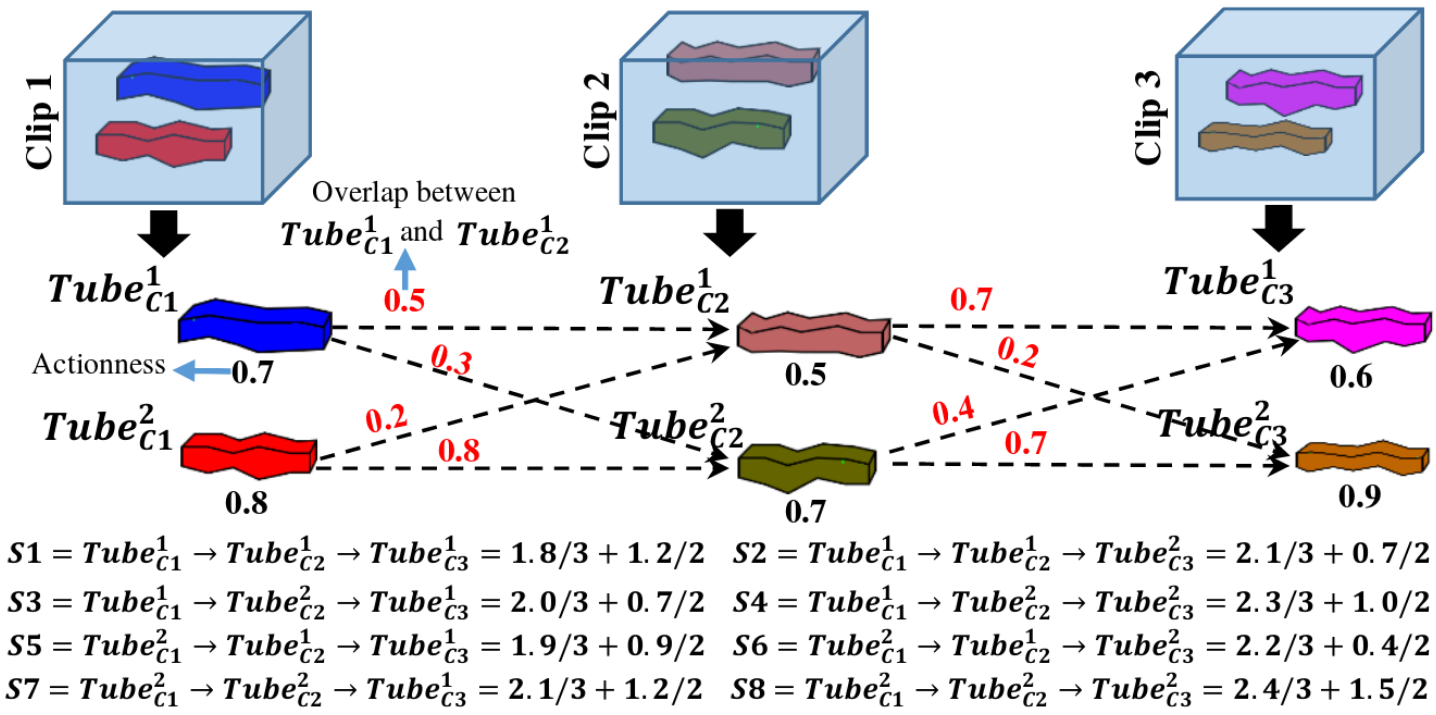
\includegraphics[scale=0.225]{connection_algo}
  \caption{An example of calculating connection score for 3 random TOIs taken from \cite{DBLP:journals/corr/HouCS17}}
  \label{fig:connection_algo}
\end{figure}

The above approach, however, needs too much memory for all needed calculations, so a memory usage  problem is
appeared. The reason is, for every new video segments we propose \textit{k TOIs} (16 during training and 150 during validation).
As a result, for a small video seperated in  \textbf{10 segments}, we need to calculate 
\textbf{  150\textsuperscript{10} scores} during validation stage. This causes our system to overload and it takes too much time to process
just one video. \par

In order to deal with this problem, we create a greedy algorithm in order to find the candidates tubes. Inituitively, this algorithm after
a new video segment keeps tubes with score higher than a threshold, and deletes the rest. So, we don't need to calculate combinations with
very low score. We wrote code for calculating tubes' scores in CUDA language, which has the ability to
parallel process the same code using different data. Our algorithm is described below:

\begin{enumerate}
\item Firstly,  initialize empty lists for the final tubes, final tubes' duratio, their scores, active tubes, their correnspondig duration,
  active tubes' overlapping sum and actioness sum where:
  \begin{itemize}
  \item Final tubes list contains all tubes which are the most likely to contain an action, and their score list contains their
    corresponding scores. We refer to each tube by its index which is related a tensor, in which we saved all the ToIs proposed
    from TPN for each video segment.
  \item Active tubes list contains all tubes that will be match with the new TOIs. Their overlapping sum list and actioness sum list
    contain their sums in order to avoid calculating then for each loop. 
  \end{itemize}
Also, we initialize threshold equal to 0.5 .
\item For the first video segment, we add all the TOIs to both active tubes and final tubes. Their scores are only their actioness because
  there are no tubes for calculating their overlapping score. So, we set their overlaping sum equal to 0.
\item For each next video, after getting the proposed ToIs, firstly we calculate their overlapping score with each active tube. Then, we
  empty active tubes, active tubes' duration, overlapping sum and actioness score lists.  For each new tube that has score higher than the threshold
  we add both to final tubes and to active tubes, and we increase their duration.
\item If the number of active tubes is higher than a threshold, we set the threshold equal to the score of
  the 100th higher score. On top of that, we update the final tubes list, removing all tubes that have score lower than the threshold.
\item After that, we add in active tubes, the current video segment's proposed TOIs. Also their actioness scores in actioness sum list and
  zero values in corrensponding positions in overlaps sum list (such as in the 1st step).
\item We repeat the previous 3 steps until there is no video segment left.
\item Finally, as we mentioned before, we have a list which contains the indexes of the saved tubes. So, we modify them in order to have
  the final bounding boxes. However, 2 succeeding ToIs do not have extactly the same bounding boxes in the frames that overlap. For example,
  ToIs from the $1^{st}$ video segment start from frame 1 to frame 16. If we have video step equal with 8, it overlaps with the ToIs from the
  succeeding video segment in frames 8-16. In those frames, in final tube, we choose the area that contains both bounding boxes which is
  denoted as $(min(x_1,x'_1), min(y_1,y'_1), max(x_2,x'_2), max(y_2,y'_2))$ for bounding boxes $(x_1,y_1,x_2,y_2)$ and $(x'_1,y'_1,x'_2,y'_2)$.
\end{enumerate}

Μερικά ενδεικτικά αποτελέσματα
sample duration 16
sample duration 8

\subsection {UCF Dataset}
enas pinakas me ola

\section{second approach}

\section{third approach}
enas pinakas


\end{document}